\documentclass[english]{article}
\usepackage[usenames,dvipsnames,svgnames,table]{xcolor}
\usepackage{babel,blindtext}
\usepackage{graphicx}
\usepackage{caption}
\usepackage{subcaption}
\usepackage{tabularx}
\usepackage{amsmath}
\usepackage{mathrsfs}
\usepackage{setspace}
\usepackage{enumerate}
\usepackage{todonotes}
\usepackage{listings}
\usepackage{paralist}
\usepackage{natbib}
\usepackage{fullpage}
\usepackage[T1]{fontenc}
\usepackage{booktabs}
\usepackage{pgfplotstable}
\usepackage{makecell}
\usepackage{comment}
\usepackage{gensymb}

\usepackage[colorlinks=true,
            linkcolor=blue,
            urlcolor=blue,
            citecolor=blue,
            final,
            hypertexnames=false]{hyperref}

%
%
%
\title{\bf{SoV Scaling Study}}
\author{Nicholas Malaya, Robert D. Moser \\ Institute for Computational Engineering and Sciences \\ University of Texas at Austin} \date{}

\begin{document}
\maketitle

\section*{System Configurations}

\begin{table}
\begin{centering}
  \begin{tabular}{ | l || c | r | r | r | r |}
    \hline     
    Case & $r_{ib}$ & $r_{it}$ & $r_{o}$ & $z_{b}$ & $z_{t}$ \\ \hline \hline
    1m   & 0.16     & 0.33     & 0.50    & 0.066   & 0.55 \\ \hline
    3m   & 0.50     & 1.00     & 1.50    & 0.200   & 1.65 \\ \hline
    5m   & 0.75     & 1.50     & 2.50    & 0.333   & 2.75 \\
    \hline 
  \end{tabular}
  \caption{The three different vane configurations. $r_{ib}$ is the inner radius of the bottom tier, 
    $r_{it}$ the inner radius of the top tier, and $r_{o}$ the outer radius (shared by both tiers). 
    $z_{b}$ and $z_{t}$ are the heights of the top and bottom tiers, respectively. }\label{fig:scaling_table}
\end{centering}
\end{table}
%

\begin{figure}[!htb]
  \begin{center}
    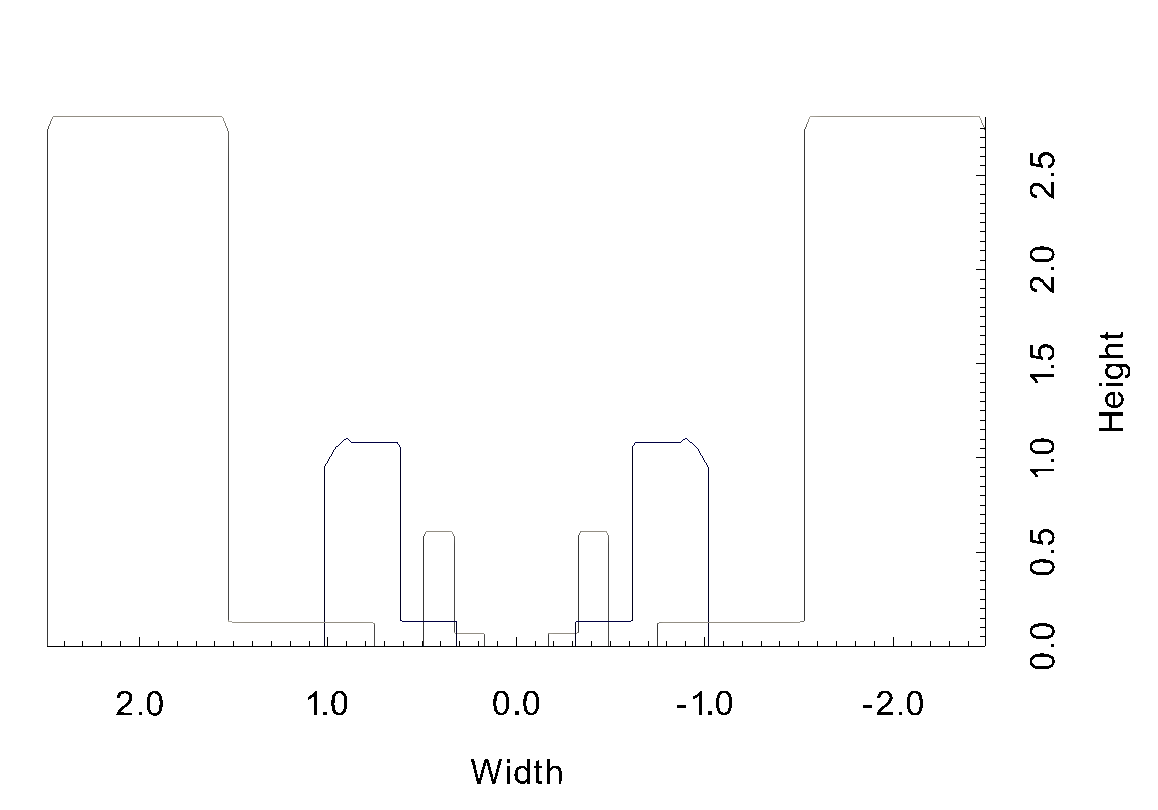
\includegraphics[width = 12 cm]{figs/vane_scaling}
    \caption{An image showing the three different vane configurations. The three-meter vanes (mid-sized set) 
      have a slight plotting artifact at the top outer corner, but this does not exist in the simulations. }
    \label{vane_scaling}
  \end{center}
\end{figure}


This document details investigations into the variation of the Solar Vortex (SoV) physical size and energy as a function of diameter of the apparatus. We consider 
three fully developed, averaged runs for system configurations that are identical excepting having been scaled to larger sizes. We will use 
system apparatus that have diameters of one, three and five meters. The design is two tiers, with a longer curved vane on the bottom tier providing a 
smoother and slower variation in angle as a function of radius. Each configuration has an outer angle of $0\degree$, and varying along a smooth curve 
depending on the square root of the radius inward to a maximum angle of $75\degree$. The ``baseline'' configuration was the three meter design, 
which was optimized over the coarse of a parameter sweep across inner and outer radius, heights, angles, etc. These different run 
definitions are completely defined in Table \ref{fig:scaling_table}. The results shown here are all temporally averaged, and are not sensitive to changes in the domain size.

%
% image of vane angle?
%
Figure \ref{vane_scaling} plots a vertical slice through the three vane sizes, to give the reader a sense of the 
scale between each configuration.

\begin{figure}[!htb]
\minipage{0.32\textwidth}
  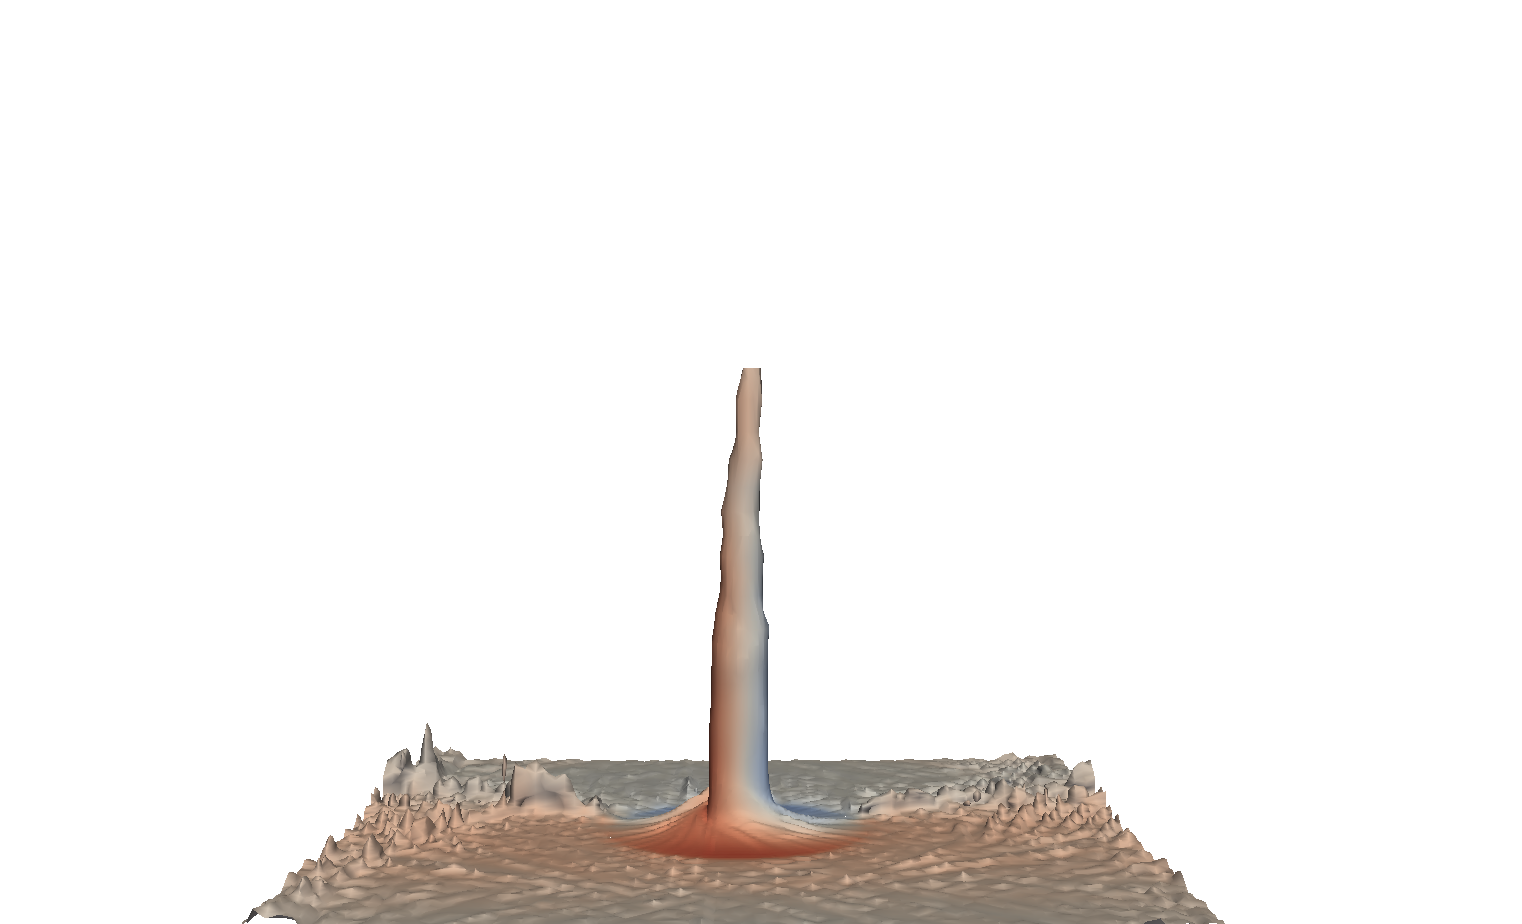
\includegraphics[width=\linewidth]{figs/1m_temp_iso}
  \caption*{1m Apparatus}\label{fig:1m_scaling}
\endminipage\hfill
\minipage{0.32\textwidth}
  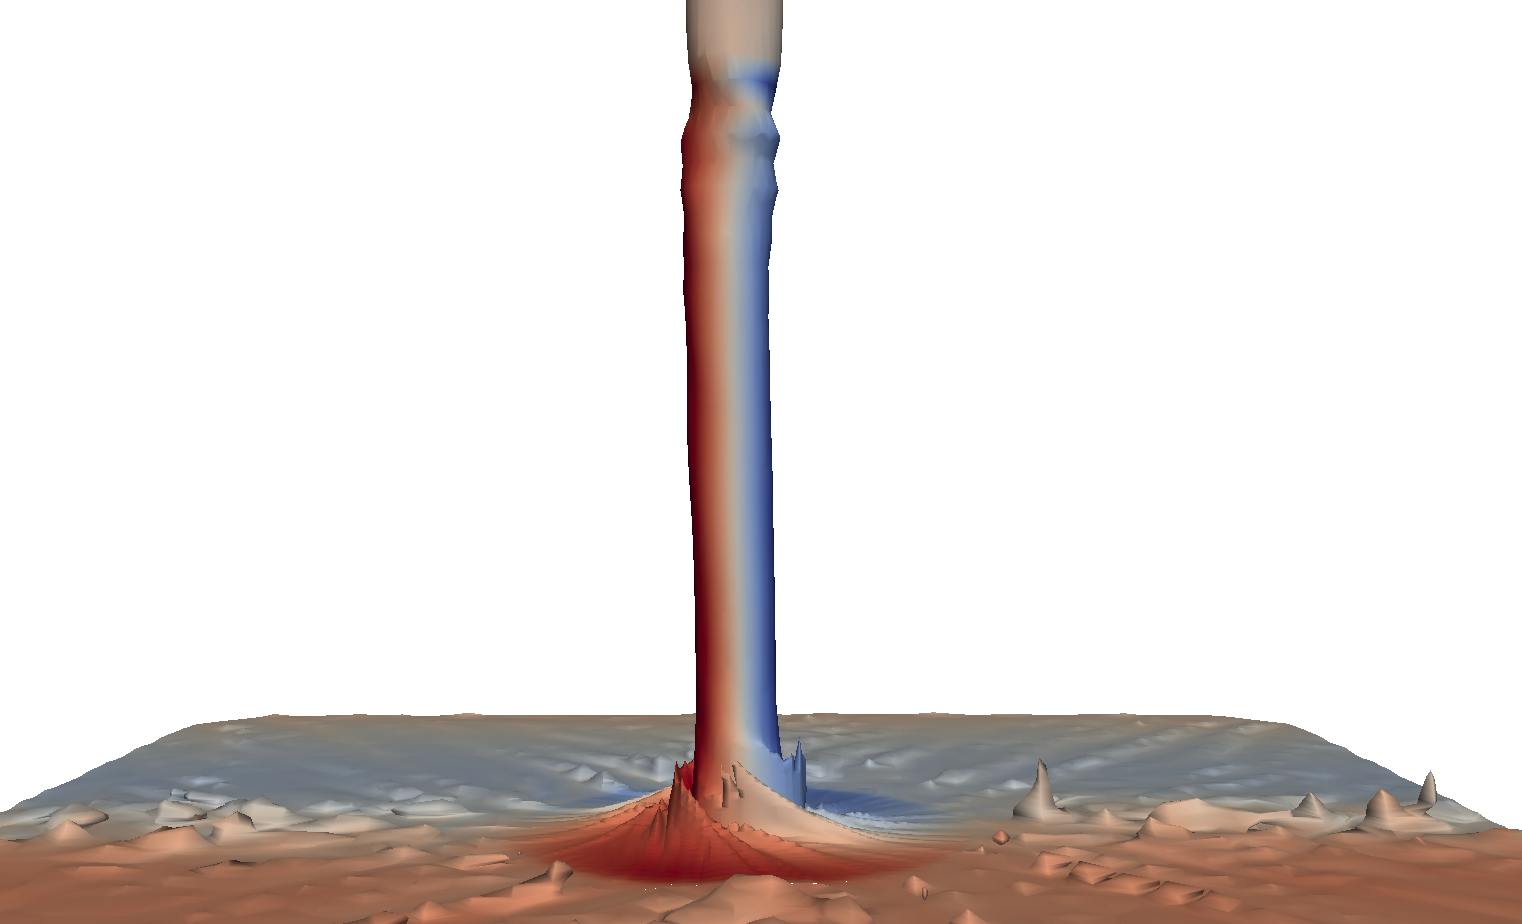
\includegraphics[width=\linewidth]{figs/3m_temp_iso}
  \caption*{3m Apparatus}\label{fig:3m_scaling}
\endminipage\hfill
\minipage{0.32\textwidth}%
  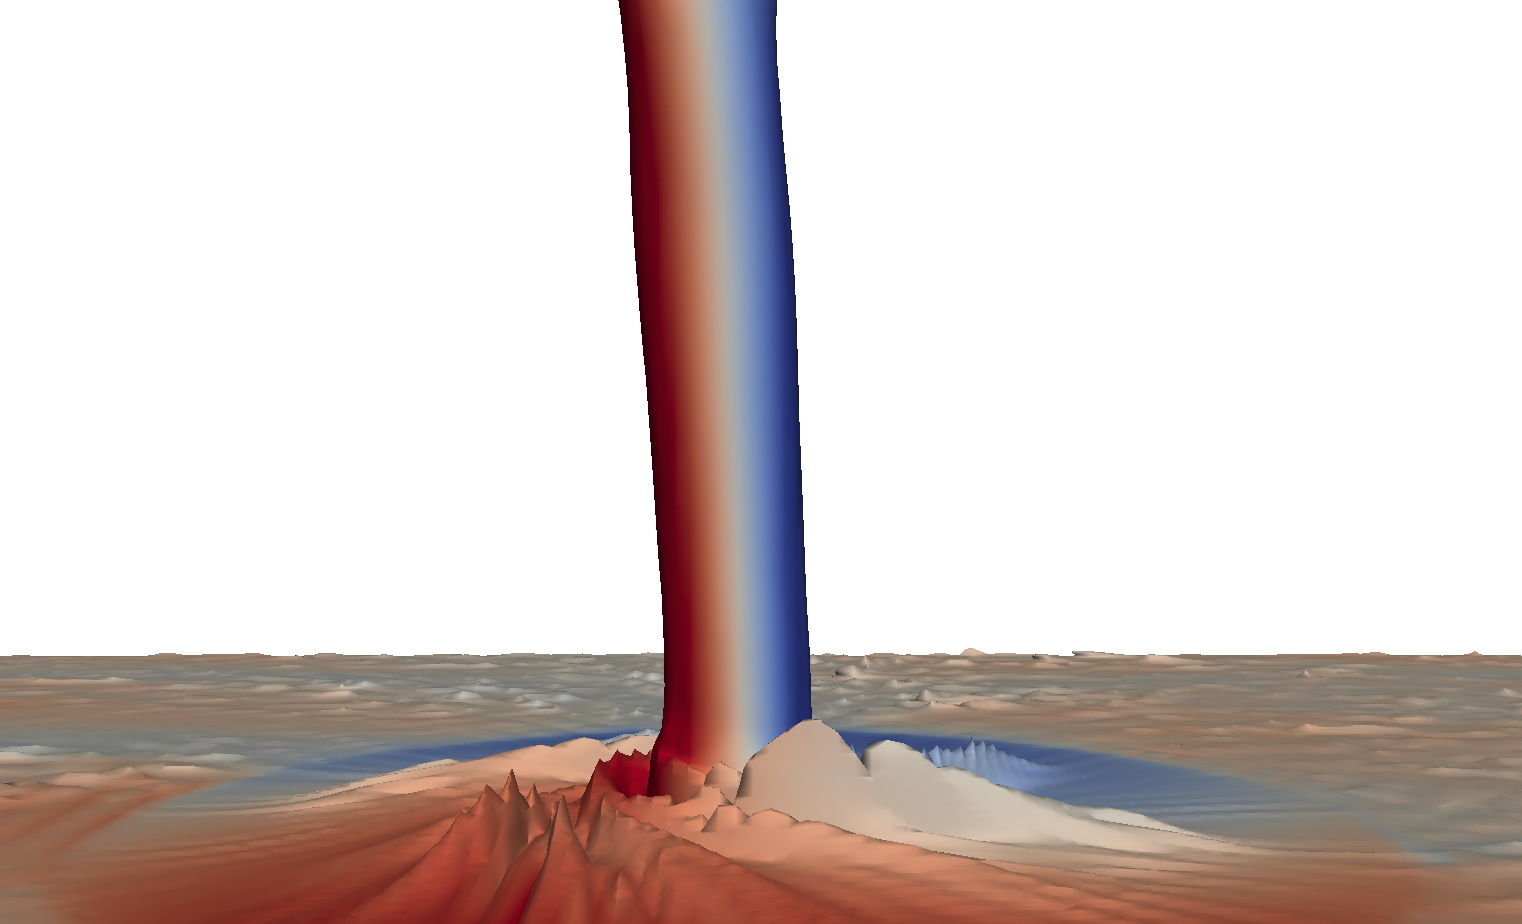
\includegraphics[width=\linewidth]{figs/5m_temp_iso}
  \caption*{5m Apparatus}\label{fig:5m_scaling}
\endminipage
\caption{3d Isocontour Rendering of the Thermal Plume across three different cases.}
\end{figure}


\begin{figure}[!htb]
  \begin{center}
    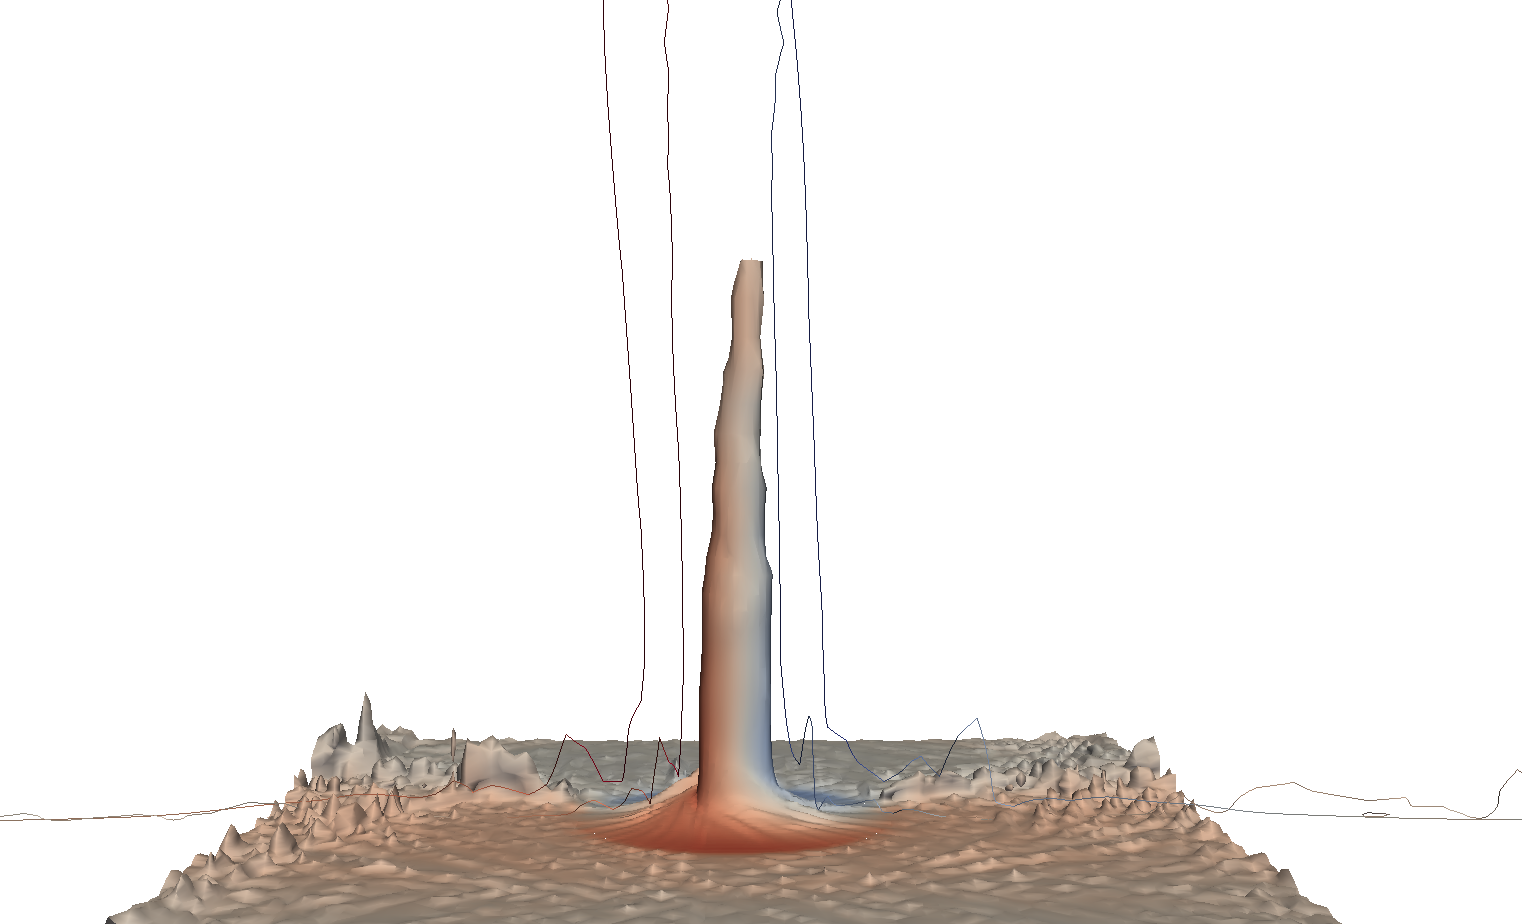
\includegraphics[width = 12 cm]{figs/temp_iso}
    \caption{Thermal Isocontours from the three different cases superimposed 
      on top of each other to show the growing extend of the thermal column at larger vane sizes. }
    \label{fig:scaling_slice}
  \end{center}
\end{figure}

\begin{figure}[!htb]
  \begin{center}
    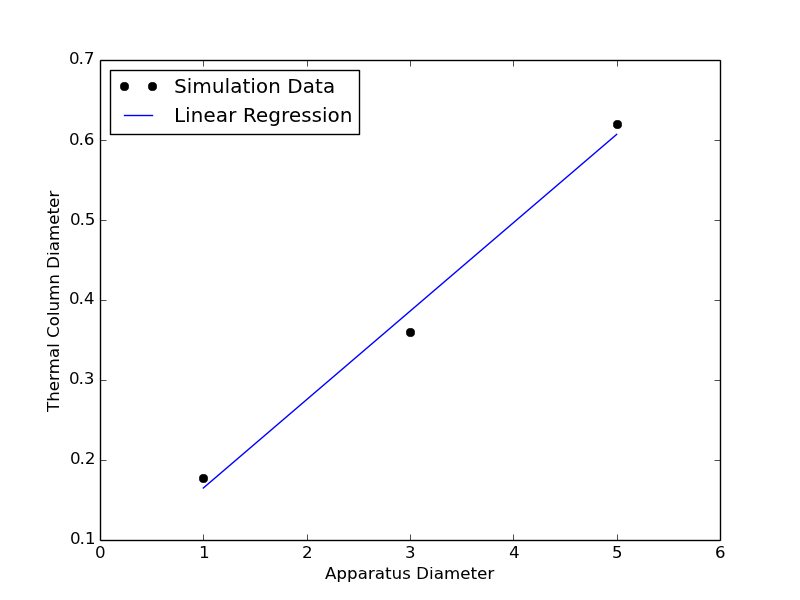
\includegraphics[width = 12 cm]{figs/scaling_regression}
    \caption{The thermal column thickness plotted against the total system diameter sizes. A linear regression is also shown against the data.}
    \label{fig:scaling_reg}
  \end{center}
\end{figure}

\section*{Thermal Plume Scaling}
Isocontours of the temperature field (contoured at 317 Kelvin) are shown in figures \ref{fig:1m_scaling}-\ref{fig:5m_scaling}. 
It is clear that as the vanes grow in size, the physical size of the thermal plume also increases. This is shown slightly more clearly in
 Figure \ref{fig:scaling_slice}. Here, the two larger cases isocountours are sliced and transparent so that one can see an approximate 
location of the thermal column thickness for each of the three cases. These thicknesses have been extracted and plotted as a 
function of outer system diameter in Figure \ref{fig:scaling_reg}, where it is clear that the trend is generally linear. It appears then that 
the thickness of the thermal plume is scaling roughly proportionally with the system outer diameter. 

%
% probably need to plot the increase in diameter as a function of diameter 
%


\begin{figure}[!htb]
\minipage{0.32\textwidth}
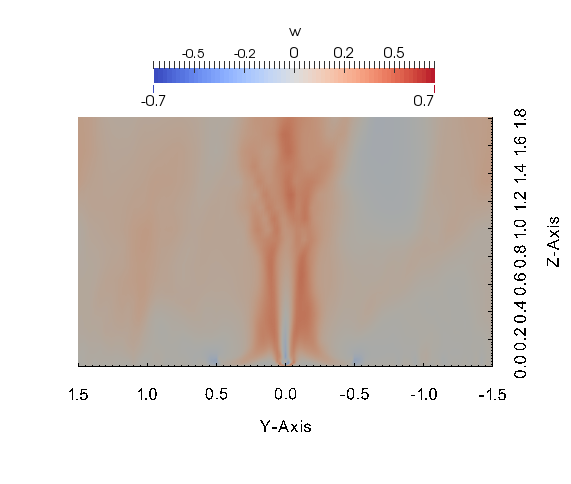
\includegraphics[width=\linewidth]{figs/w_scaled_1m}
\caption*{1m}\label{fig:1m_vz}
\endminipage\hfill
\minipage{0.32\textwidth}
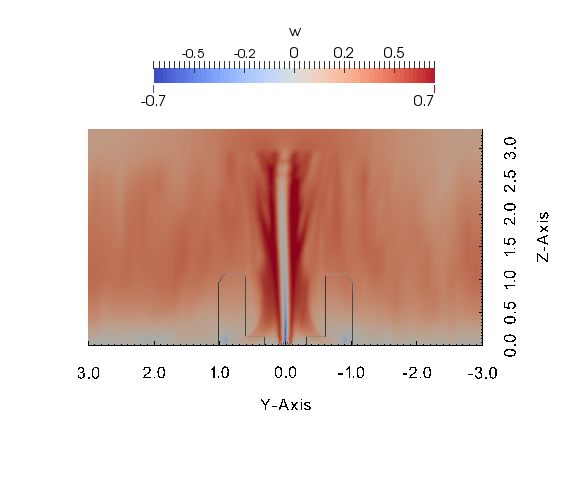
\includegraphics[width=\linewidth]{figs/w_scaled_3m}
\caption*{3m}\label{fig:3m_vz}
\endminipage\hfill
\minipage{0.32\textwidth}%
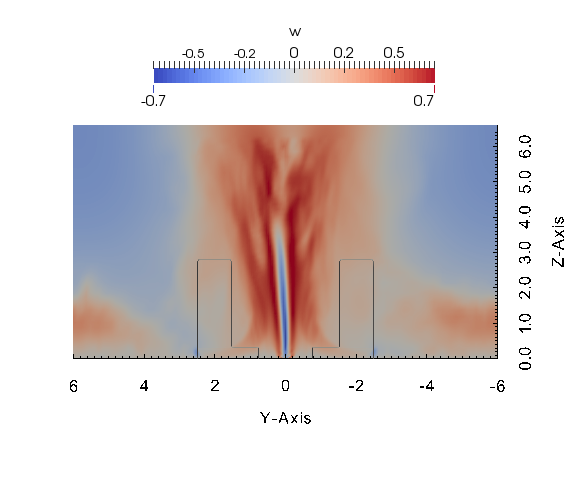
\includegraphics[width=\linewidth]{figs/w_scaled_5m}
  \caption*{1m}\label{fig:5m_vz}
\endminipage
\caption{Vertical Velocity}
\end{figure}
 
Figure \ref{fig:scaling_slice} shows the vertical velocity for each of the three cases. In each case the aspect ratio between domain extent
and apparatus size are maintained roughly constant, so as to give the appearance of ``scaling'' each apparatus. In this way, it is more 
clear here than in the thermal column case that there exists a qualitatively similar structure between each of the three cases. The velocity plume 
size occupies roughly the same fraction of the volume inside the vanes. 

For these three cases, we calculate the kinetic energy flux as, 
\begin{equation}
k = \frac{1}{2} \int v_z (v_z^2 + v_{\theta}^2) dA. 
\label{ke_flux}
\end{equation}

%Where the Kinetic energy flux for the 1m,3m and 5m are then 

%
% just a figure
%

  %% \begin{figure}[!htb]
  %%   \begin{center}
  %%    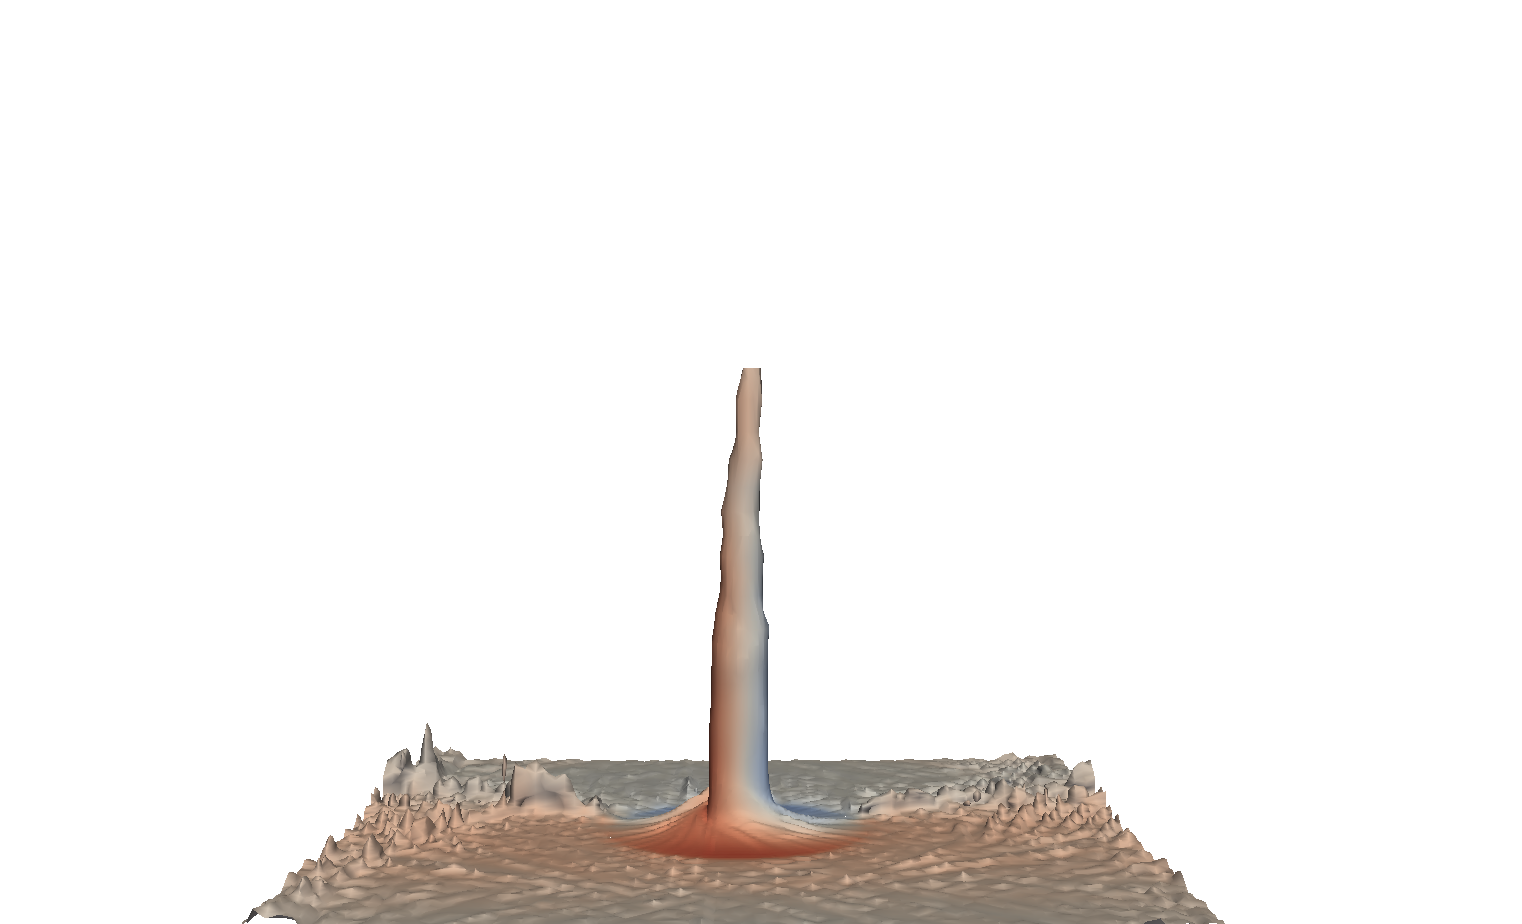
\includegraphics[width = 12 cm]{figs/1m_temp_iso}
  %%    \caption{1m }
  %%    \label{lab}
  %%   \end{center}
  %% \end{figure}
\section*{Predictions for System Scaling}

%We can use our model to make some very rough predictions for system sizes to attain various power outputs. 

A crucial question now is how do we expect the kinetic energy to scale with larger system sizes. We expect the 
kinetic energy to scale with some unknown exponent of the diameter, 
\begin{equation}
k \propto D^\alpha. 
\end{equation}

\begin{figure}[!htb]
  \begin{center}
    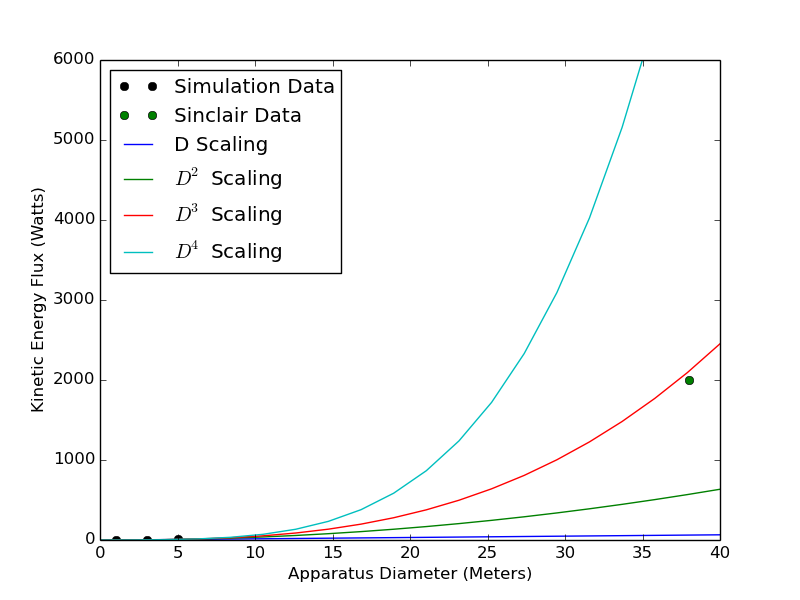
\includegraphics[width = 12 cm]{figs/ke_regression}
    \caption{The kinetic energy fluxes for the three configurations extrapolated out to larger configuration sizes.}
    \label{fig:ke_regression}
  \end{center}
\end{figure}

An interesting question is to ask if these predictions are consistent with the available experimental results. 
Sinclair (1973) has experimentally measured profiles, which can be integrated using equation \ref{ke_flux} to 
provide an estimate of the energy flux. This is measured to be $\approx 2.4$ kW. Examining the thermal 
profiles from Sinclair, the thermal plume thickness is found to be roughly 4.6 meters in diameter. This is 
7.6 times larger than the thermal plume thickness measured in the five-meter configuration. If we assume 
linear scaling in vane configurations, that would require a 38 meter outer diameter configuration to 
generate the same energy flux as the Sinclair field dust-devils. Figure \ref{fig:ke_regression} shows 
several powers of extrapolations from the present data sets to the larger diameter sizes. Our projections 
are roughly consistent with the Sinclair data for a scaling coefficient between three and four. 

\end{document}
